\documentclass[11pt,letterpaper,english]{article}

\usepackage[margin=1.0in]{geometry}
\usepackage{helvetica}
\usepackage{graphicx}

\title{Monsanto's Earning Announcement}
\author{Ian Clark}
\date{}

\begin{document}
\maketitle

\section{Results of the Earnings Report Upon the Market} 
The market opened with news of Monsanto's Earnings Report readily available causing a rise--a $\Delta{P_{MON}} = 1.54 $--between the dates of 31 March 2015 and 01 April 2015--01 April being the date where the earnings report was made available. As indicated by the chart below, we can see that Monsanto's stock price was much more volatile than in the nearly two weeks prior.

\begin{center}
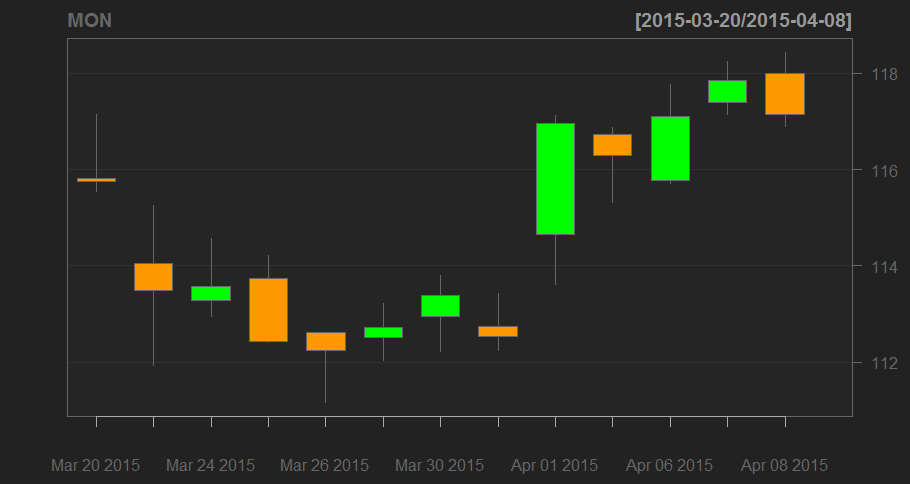
\includegraphics[scale=0.5]{Data/CandleChart.png}
\end{center}

\section{Earnings per Share}
By Monsanto's estimates, their Earnings per Share ($2.92 \$ $) has reamained within their estimates, but fallen over the course of the year toward the lower end of their acceptable range. A factor assumed to be heavily affecting both Monsanto and the US economy as a whole is the strengthening of the dollar in relations to other currencies--notably the Euro.

\vspace{0.5mm}
\noindent


\newpage
\begin{thebibliography}{9}
\bibitem{Monsanto Earnings Presentation}
    Monsanto,
    \emph{$http://www.monsanto.com/investors/documents/2015/2015.04.01_mon_q2fy15_earnings.pdf$}.
\bibitem{Yahoo Finance Coverage of Report}
     Yahoo Finance,
     \emph{$http://finance.yahoo.com/news/monsanto-announces-second-quarter-financial-120000678.html$}
\end{thebibliography}

\end{document} 